\documentclass[%
 reprint,
 superscriptaddress,
 amsmath,
 amssymb,
 prl,
]{revtex4-1}

\usepackage{graphicx}% Include figure files
\usepackage{dcolumn}% Align table columns on decimal point
\usepackage{bm}% bold math

\begin{document}

\title{Arrival Time Stabilisation of a Relativistic Electron Beam at 
the 50~fs Level}

\author{J.~Roberts}
\email{Corresponding author Jack.Roberts@cern.ch}
\affiliation{John Adams Institute (JAI), University of Oxford, Denys Wilkinson 
Building, Keble Road, Oxford, OX1 3RH, United Kingdom}
\affiliation{The European Organization for Nuclear Research (CERN), Geneva 23, 
CH-1211, Switzerland}

\author{P.~Skowronski}
\affiliation{The European Organization for Nuclear Research (CERN), Geneva 23, 
	CH-1211, Switzerland}

\author{P.~Burrows}
\affiliation{John Adams Institute (JAI), University of Oxford, Denys Wilkinson 
Building, Keble Road, Oxford, OX1 3RH, United Kingdom}

\author{G.~Christian}
\affiliation{John Adams Institute (JAI), University of Oxford, Denys Wilkinson 
Building, Keble Road, Oxford, OX1 3RH, United Kingdom}

\author{R.~Corsini}
\affiliation{The European Organization for Nuclear Research (CERN), Geneva 23, 
CH-1211, Switzerland}

\author{A.~Ghigo}
\affiliation{Laboratori Nazionali di Frascati (LNFN), Via Enrico Fermi, 40, 
00044 
Frascati RM, Italy}

\author{F.~Marcellini}
\affiliation{Laboratori Nazionali di Frascati (LNFN), Via Enrico Fermi, 40, 
00044 
Frascati RM, Italy}

\author{C.~Perry}
\affiliation{John Adams Institute (JAI), University of Oxford, Denys Wilkinson 
Building, Keble Road, Oxford, OX1 3RH, United Kingdom}


\date{\today}

\begin{abstract}
CLIC, a proposed future linear electron-positron collider, and other machines 
such as XFELs, place tight tolerances on the phase stabilities of their beams. 
CLIC proposes the use of a novel, high bandwidth and low latency, `phase 
feedforward' system required to achieve a phase stability of 
\(0.2^\circ\)~at~12~GHz, or about 50~fs. This work documents the results from 
operation of a prototype phase feedforward system at the CLIC test facility 
CTF3, with \(>23\)~MHz bandwidth and a total hardware latency of 100~ns. New 
phase monitors with 30~fs resolution, 20~kW amplifiers with 47~MHz bandwidth, 
and electromagnetic kickers have been designed and installed for the system. 
The system utilises a dog-leg chicane in the beamline, for which a dedicated 
optics have been created and commissioned. The prototype has demonstrated 
CLIC-level phase stability, reducing an initial rms phase variation of 
\(0.92\pm0.04^\circ\) to \(0.20\pm0.01^\circ\).
\end{abstract}

\maketitle

The Compact Linear Collider, CLIC, \cite{CLICCDR} is a proposed future 
linear electron--positron collider. It uses a novel two beam acceleration 
concept to achieve a high accelerating gradient of 100~MV/m 
and a collision energy of up to 3 TeV. In this concept the 12~GHz RF power used 
to accelerate each high energy colliding beam is extracted and transferred from 
a high intensity drive beam in 24 decelerator sectors. The 
drive beams are generated by compressing an initial 
\(140~\mathrm{\mu s}\) beam pulse bunched at 0.5~GHz into 24 shorter 240~ns 
beam pulses bunched at 12~GHz, in a bunch recombination process using a 
sequence of combiner rings and delay loops \cite{CLICCDR}.

CLIC's luminosity quickly drops if the drive beam phase, or arrival time, 
jitters with respect to the colliding beams, causing energy errors and 
subsequent beam size growth at the interaction point. The drive beam phase 
stability must be \(0.2^\circ\)~at~12~GHz (around 50~fs) rms or better to limit 
the luminosity loss to below 1\% \cite{CLICCDR}.  However, the drive beam phase 
stability cannot be guaranteed to be better than \(2^\circ\)~at~12~GHz 
\cite{CLICCDR}. A 
mechanism to improve the drive beam phase stability by an order of magnitude is 
therefore required. The correction must be applied to the full drive beam pulse 
length and have a bandwidth exceeding 17.5~MHz to achieve this 
\cite{Gerber2015}. Higher frequency errors are filtered as a consequence of the 
drive beam recombination process, and by the accelerating structures 
\cite{Gerber2015}.

Other machines, such as XFELs, have similar beam phase stability 	
requirements to CLIC. At FLASH, DESY, these requirements have been met using 
an RF phase and power feedback based on the measurement of electro-optic beam 
arrival time monitors \cite{flashPRL}. 
FLASH has 1~MHz bunch spacing and a 500~ms beam pulse, whereas the CLIC drive 
beam has 12~GHz bunch spacing and 240~ns pulse length. A feedback with a 
latency of several microseconds is therefore not suitable for CLIC.

Instead, a drive beam ``phase feedforward'' (PFF) 
system is proposed. A prototype PFF system, following the same concept as the 
CLIC proposal, has been designed, commissioned and operated at 
the CLIC test facility CTF3, at CERN, to prove its feasibility. CTF3 provides a 
135~MeV electron beam bunched at 3~GHz with a pulse length of 1.2~\(\mathrm{\mu 
s}\) and a pulse repetition rate of 0.8~Hz \cite{CLICCDR}. All phases quoted in 
the paper are given in degrees at 12~GHz, as relevant for CLIC.

\begin{figure}
	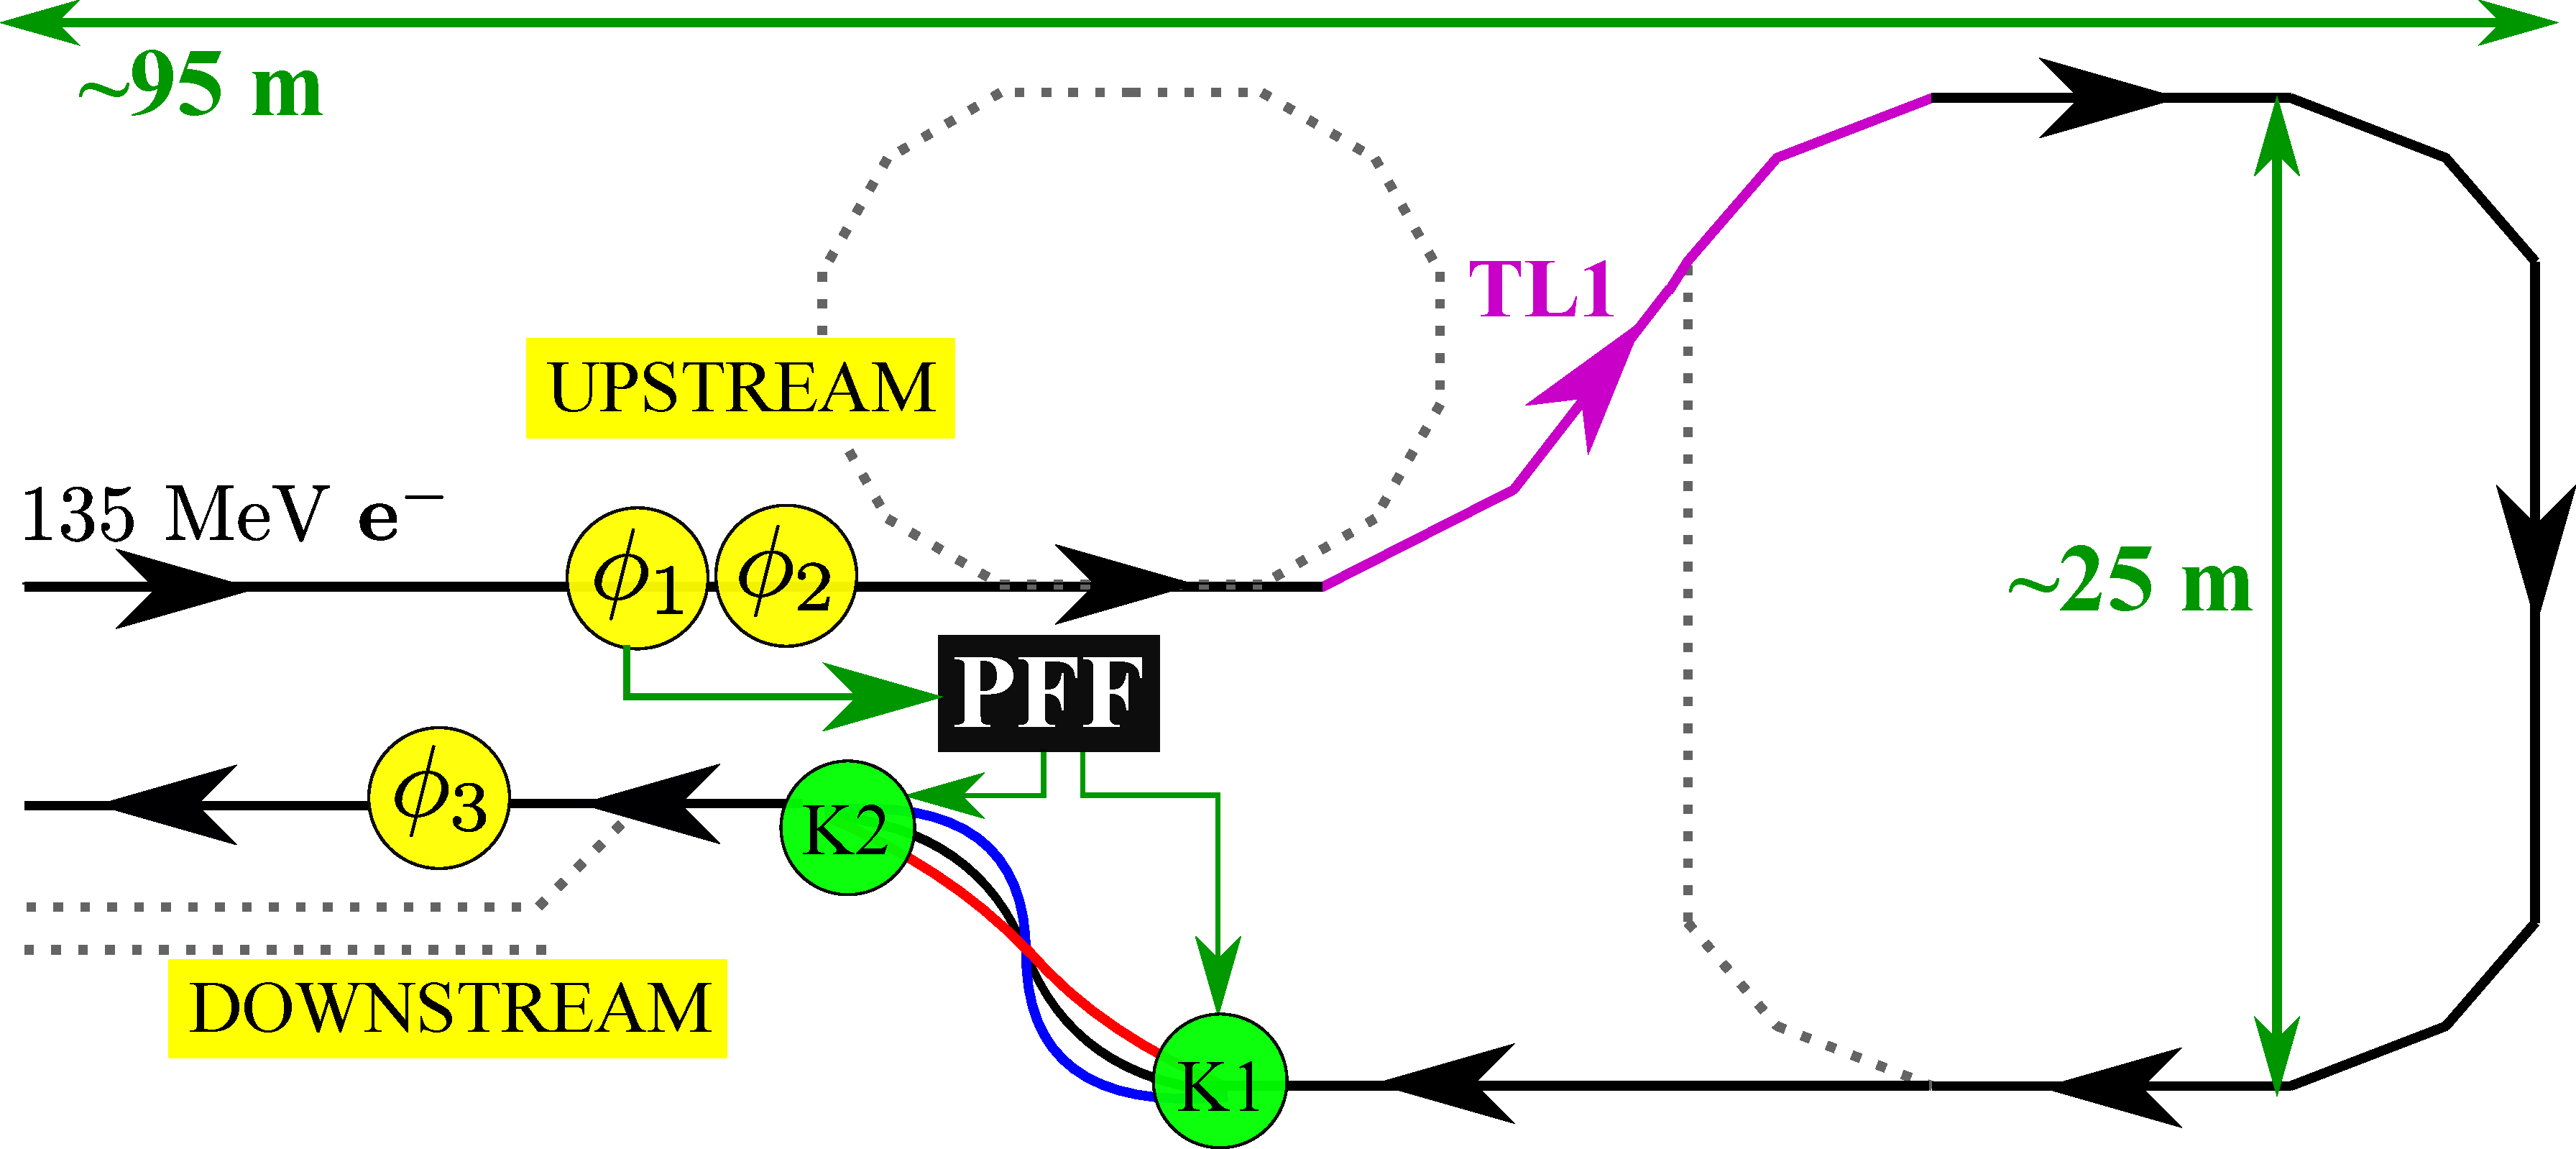
\includegraphics[width=\columnwidth]{figs/ctfpffLayout}% Here is 
	%how to 
	%import EPS art
	\caption{\label{fig:pffLayout}Schematic of the PFF prototype at CTF3, 
	showing the phase monitors (\(\phi_1\) , 
	\(\phi_2\) and \(\phi_3\)) and kickers (K1 and K2). The black box “PFF” 
	represents the calculation and output of the correction, including the 
	phase monitor electronics, feedforward controller and kicker amplifiers.
	Dashed lines indicate beam lines that are not used during PFF operation. 
		}
\end{figure}

A schematic of the prototype PFF system is shown in Fig.~\ref{fig:pffLayout}. 
The system corrects the phase using two electromagnetic kickers installed 
before the first and last dipole in a four bend, dog-leg shaped chicane. The 
beam's path length through the chicane depends on the voltage applied to the 
kickers. Bunches arriving early at the upstream 
phase monitor are deflected on to longer trajectories 
in the chicane, and bunches arriving late on to shorter trajectories. 
Downstream of the chicane another phase monitor is placed to measure the 
effects of the correction.

The beam time of flight between the upstream phase monitor and the first kicker 
in the chicane is 380~ns. The total cable length for the PFF correction signals 
is shorter, around 250~ns (see Fig.~\ref{fig:pffLayout}). The PFF correction in 
the chicane can therefore be applied to the same bunch initially measured at 
the phase monitor, providing the total system hardware latency is less than 
130~ns. 

The PFF system presents a significant hardware challenge, in particular in 
terms of the power, latency and bandwidth requirements for the kicker 
amplifiers, and the resolution and bandwidth of the phase monitors. A low 
latency digitiser and feedforward controller is also required.
Table~\ref{tab:pffspecs} compares the requirements of the CLIC system and their 
corresponding values at CTF3. 
The main differences result from the different drive beam energies, and scales 
of the two facilities. Higher power amplifiers (500~kW rather than 20~kW) are 
required at CLIC, which may be achieved by combining the output of multiple 
modules similar to the CTF3 design. CLIC also requires the 
synchronisation of multiple PFF systems distributed along the 50~km facility, 
which is not addressed by the CTF3 prototype (see \cite{CLICCDR}).

\begin{table}
	\caption{\label{tab:pffspecs}
	    Requirements for the proposed CLIC PFF system, and how they compare to 
	    the parameters and achievements of the prototype at CTF3.}
\begin{ruledtabular}
	\begin{tabular}{lccc}
		 & CLIC & CTF3 \\
		\hline
		Drive Beam Energy & 2400 & 135 & MeV \\
		No. PFF Systems & 48 & 1 & \\
		Kickers per PFF Chicane & 16 & 2 & \\
		Power of Kicker Amplifiers & 500 & 20 & kW \\
		Angular Deflection per Kicker & \(\pm94\) & 
		\(\pm560\) & \(~\mathrm{\mu rad}\) \\
		Correction Range & \(\pm 10\) & \(\pm 6\) & \(^\circ\) \\
		Correction Bandwidth & \(>17.5\) & \(>23\) & MHz \\
		Phase Monitor Resolution & \(< 0.14\) & \(0.12\) &  \(^\circ\)   \\
		Initial Phase Jitter & \(2.0\) & \(0.9\) &  \(^\circ\)  \\
		Corrected Phase Jitter & \(0.2\) & \(0.2\) &  \(^\circ\)  \\
	\end{tabular}
\end{ruledtabular}
\end{table}

The hardware at CTF3 has been designed and constructed by a collaboration 
between CERN, the John Adams Institute/Oxford University, and INFN Frascati.

The phase monitors \cite{phMonEuCard} are cylindrical cavities with an aperture 
of 23~mm and a length of 19~cm. Notch filters, small ridges, in the cavity 
create a resonating volume at 12~GHz, whilst also reflecting stray fields.
The fields induced by the beam traversing the cavity contain a position 
independent monopole mode and a position dependent dipole mode. The unwanted 
position dependence is removed by summing the output from an opposing pair 
of feedthroughs, on the top and bottom of the cavity, in a hybrid. 
To extract the beam phase the output from the hybrids 
is mixed with a 12~GHz reference signal, derived from a 3~GHz source 
time-locked to CTF3 and common to all three phase monitors.
In the electronics for each phase monitor the beam and reference signals are 
split between eight separate mixers, with the output from each combined to give 
the final phase dependent outputs. This has allowed a resolution of 
\(0.12^\circ\), or about 30~fs, to be achieved whilst maintaining linearity 
between \(\pm70^\circ\) \cite{RobertsThesis}. The quoted resolution 
is determined by comparing the measurements of the two adjacent upstream 
monitors (see Fig.~\ref{fig:pffLayout}).

The kicker amplifiers \cite{RobertsThesis} have a modular design, 
consisting of a central control module, and two drive and terminator modules 
(one per kicker). The control module distributes power and input signals to the 
drive modules. The 20~kW drive modules consist of low voltage Si FETs driving 
high voltage SiC FETs, and for an input voltage of \(\pm2\)~V give an output of 
up to \(\pm700\)~V. The output is linear within 3\% for input voltages between 
\(\pm1.2\)~V, and has a bandwidth of 47~MHz for small signal variations up to 
20\% max output. For larger signal variations the bandwidth is slew rate 
limited.

The two electromagnetic stripline kickers \cite{kickerIPAC11} are based on the 
DAFNE design \cite{dafnePAC09}. Each kicker is approximately 1~m in length, and 
has an internal diameter of 40~mm between the two strips placed along the 
horizontal walls of the device. The kickers are designed to give a fast 
response of a few ns to the input signal, and to give high kick efficiency. The 
strips have tapered ends to reduce beam coupling impedance.
A voltage of 700~V, the maximum output of the amplifiers, applied to the 
downstream ends of the kicker strips yields a horizontal deflection of 
0.56~mrad for the 135~MeV CTF3 beam.

The feedforward controller (FONT5a board) \cite{RobertsThesis} digitises the 
processed phase monitor 
signals and then calculates and outputs the appropriate amplifier input 
voltage. The FONT5a board also controls the correction timing. It consists of a 
Virtex-5 field programmable gate array (FPGA), nine 14-bit analogue to digital 
converters (ADCs) clocked at 357~MHz, and four digital to analogue converters 
(DACs). The combined hardware and firmware latency for the PFF system is 
approximately 100~ns. The output from the FONT5a board is delayed by an 
additional 30~ns to synchronise the correction at the kicker with the beam 
\cite{RobertsThesis}.

\begin{figure}
	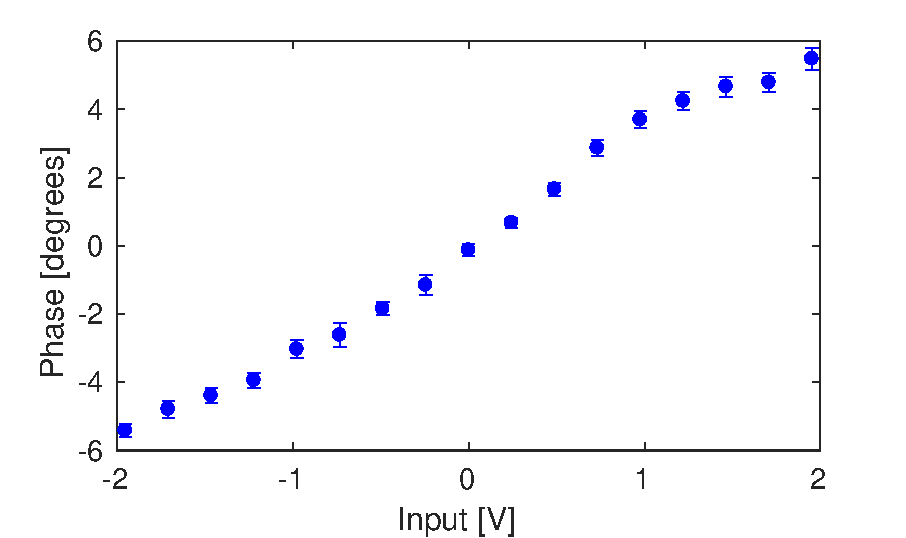
\includegraphics[width=\columnwidth]{figs/corrRange}
	\caption{\label{fig:corrRange}Downstream phase vs. the kicker amplifier 
		input voltage. Standard errors on the measured phase are shown.}
\end{figure}

As well as the hardware challenges, the PFF system places additional 
constraints on the optics of the correction 
chicane, and also on the beam lines between the upstream phase monitor and the 
chicane.
The optics transfer matrix coefficient \(R_{52}\) between the kickers relates 
the change in path length through the chicane per unit 
deflection at the first kicker. 
With an \(R_{52}\) value of \(0.74\)~m in the chicane optics 
\cite{RobertsThesis} the expectedcorrection range (path length change) of 
the PFF system is \(\pm400~\mathrm{\mu m}\), or \(\pm6^\circ\), considering the 
maximum deflection of \(\pm0.56\)~mrad from the kickers.
The measured phase shift in the chicane versus the amplifier input voltage is 
shown in Fig.~\ref{fig:corrRange}, and agrees with the expected range. 

The PFF system also should not change the beam orbit after the chicane. 
The chicane optics are designed so that the second kicker closes the orbit 
bump created by the first kicker \cite{RobertsThesis}.

One of the key challenges in operating the PFF prototype at CTF3 has been 
obtaining high correlation between the initial, uncorrected, upstream and 
downstream phase. 
A correlation of 97\% is required to reduce a typical initial 
phase jitter of \(0.8^\circ\) at CTF3 to the target of \(0.2^\circ\) 
\cite{RobertsThesis}. 
The achievable correlation depends on the phase monitor resolution and any 
additional phase jitter introduced in the beam lines between the upstream and 
downstream phase monitors. The phase monitor resolution of \(0.12^\circ\) 
limits the maximum upstream-downstream phase correlation to
\(98\%\) in typical conditions, and places a theoretical limit of
\(0.17^\circ\) on the measured corrected downstream phase 
jitter. 
Meanwhile, the dominant source of uncorrelated downstream phase jitter at CTF3 
is beam energy jitter being transformed in to phase jitter. 

\begin{figure}
	\includegraphics[width=\columnwidth]{figs/r56Scan}
	\caption{\label{fig:r56Scan}Downstream (red) and upstream (blue) phase 
	jitter vs. the \(R_{56}\) value in TL1. 
		}
\end{figure}

The first order phase-energy dependence can be described via the optics 
transfer matrix coefficient \(R_{56}\):
\(\phi_d = \phi_u + R_{56}(\Delta p / p)\)
, where \(\Delta p / p\) is the relative beam energy offset, and \(\phi_u\) and 
\(\phi_d\) are the upstream and downstream phase respectively.
Optimal conditions for the PFF system are obtained when the total \(R_{56}\) 
between the upstream and downstream monitors is zero.
To achieve this the \(R_{56}\) value in one of the transfer lines at CTF3 (TL1) 
has been tuned to compensate for non-zero \(R_{56}\) values in other lines.
Fig.~\ref{fig:r56Scan} shows that with an \(R_{56}\) of 10~cm in TL1 the 
first order phase-energy dependence is removed and the 
downstream phase jitter is reduced to the same level as the upstream jitter. 
However, a large second order phase-energy dependence remains uncorrected, and 
this leads to a degradation in upstream-downstream phase correlation if there 
are drifts in beam energy \cite{RobertsThesis}. 

Gain scans have been completed to verify the setup of the system and derive the 
optimal gain, as shown in Fig.~\ref{fig:gScan}. 
Taking in to account drifts in the initial upstream-downstream phase 
correlation and downstream phase jitter during the scan, the achieved and 
predicted performance agree within the error at all gains. 
At CTF3 the optimal system gain is typically in the range 1.0--1.2, 
being larger than unity when there is a small amplification in the downstream 
phase jitter with respect to the upstream phase jitter \cite{RobertsThesis}.

\begin{figure}
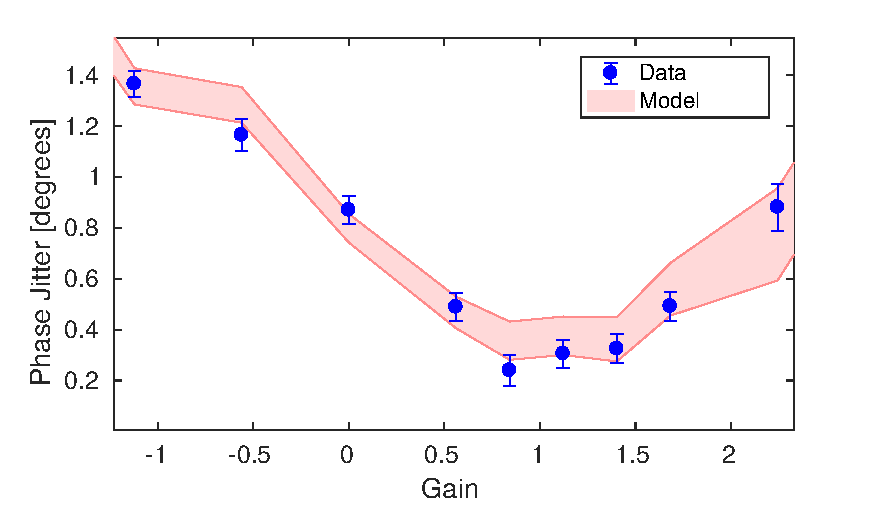
\includegraphics[width=\columnwidth]{figs/gScan}
\caption{\label{fig:gScan}Downstream phase jitter with the PFF system on at 
different gains. Markers show the measured phase jitter with standard error 
bars. The shaded red region shows the expected performance given the initial 
beam conditions.}
\end{figure}

The PFF correction is shaped to remove phase variations along the 
1.2~\(\mathrm{\mu s}\) CTF3 beam pulse. The predominant intra-pulse feature at 
CTF3 is a roughly parabolic ``phase sag'' of \(40^\circ\) peak-to-peak, 
resulting from the use of RF pulse compression \cite{CLICCDR}. As this is much 
larger than the \(\pm 6^\circ\) range of the PFF system, only approximately a 
400~ns portion of the pulse can be optimally corrected. The phase sag would not 
be present at CLIC, where in any case the drive beam pulse length is less than 
400~ns.

\begin{figure}
	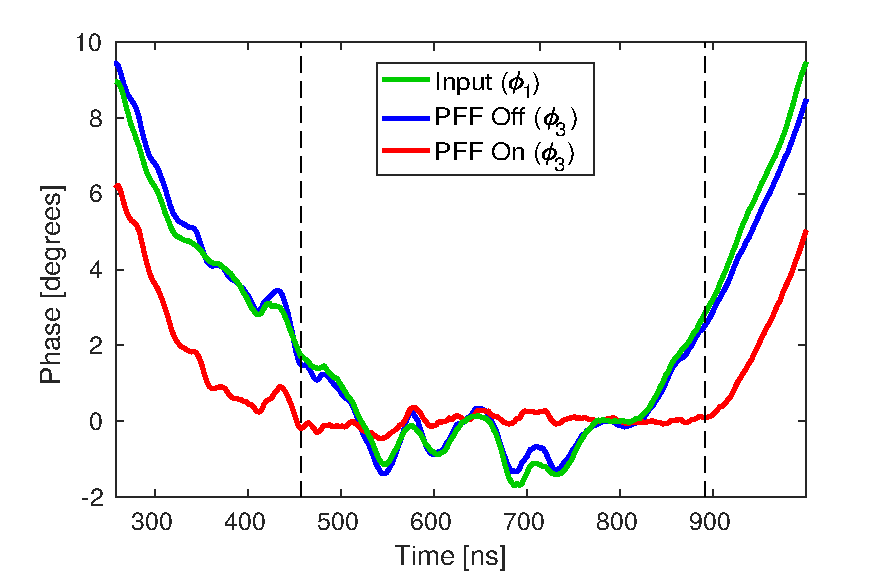
\includegraphics[width=\columnwidth]{figs/shape}
	\caption{\label{fig:shape}Effect of the PFF system on intra-pulse phase 
		variations. The pulse shapes upstream (green), and downstream with the 
		PFF 
		system off (blue) and on (red) are shown.}
\end{figure}

Fig.~\ref{fig:shape} shows the effect of the PFF system on the intra-pulse 
phase variations. The convention at CTF3 is to 
operate the PFF system in interleaved mode, with 
the correction applied to alternating pulses only. This allows a measurement of 
the initial (`PFF Off') and corrected (`PFF On') downstream phase to be 
performed concurrently. The upstream (PFF input) phase is also shown for 
comparison. Vertical dashed lines mark a 440~ns portion of the pulse where the 
correction is optimal, and this range is used to calculate statistics on the 
effect of the system. 

\begin{figure}
	\includegraphics[width=\columnwidth]{figs/fft}
	\caption{\label{fig:fft}Amplitude of phase errors at different frequencies 
		(\(f\)) with the PFF system off (blue) and on (red).}
\end{figure}

In this range the PFF system flattens the phase, 
and almost all variations are removed. Residual offsets in the phase are still 
present where there are small uncorrelated differences between the shape of the 
initial upstream and downstream phase. 
The average rms phase variation within the 440~ns range 
for each beam pulse in the dataset is reduced from \(0.960\pm0.003^\circ\) with 
the PFF system off, to to \(0.285\pm0.004^\circ\) with the system on.

CLIC requires a PFF correction with a bandwidth in excess of 17.5~MHz. 
Fig.~\ref{fig:fft} shows the effect of the PFF system on the amplitude of 
intra-pulse phase errors at different frequencies. At CTF3 there are typically 
no measurable phase errors at frequencies above 25~MHz. The PFF system is able 
to reduce the amplitude of all phase errors up to that frequency, exceeding the 
CLIC requirements. Considering the specifications of the hardware, the true 
bandwidth of the CTF3 system is believed to be above 30~MHz.

As well as removing intra-pulse phase variations the PFF system simultaneously 
corrects offsets in the overall mean phase, i.e. any pulse-to-pulse jitter. The 
mean phase of each beam pulse is calculated across the 440~ns range in the 
central portion of the pulse, as shown before in Fig.~\ref{fig:shape}.

\begin{figure}
	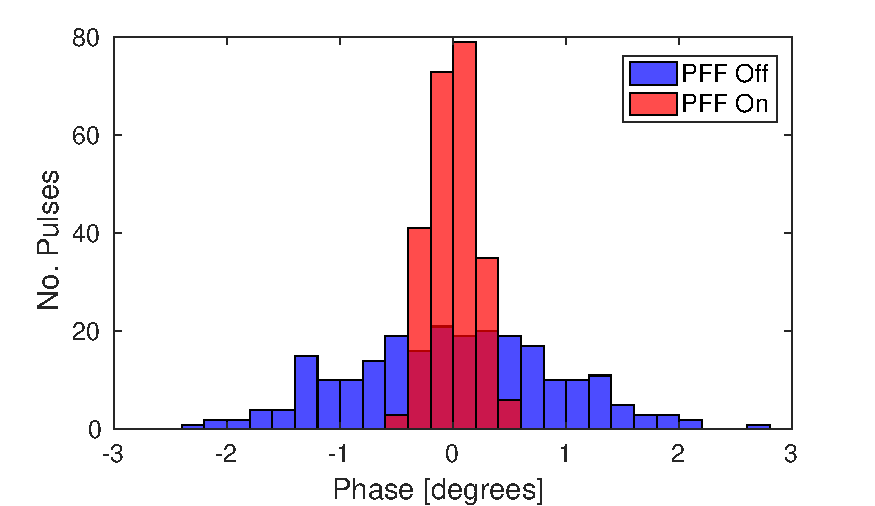
\includegraphics[width=\columnwidth]{figs/meanJit}
	\caption{\label{fig:meanJit}Distribution of the mean downstream phase with 
		the 
		PFF system off (blue) and on (red).}
\end{figure}

Fig.~\ref{fig:meanJit} shows the effect of the PFF system on the pulse-to-pulse 
stability across a dataset around ten minutes in length. An 
initial mean downstream phase jitter of \(0.92\pm0.04^\circ\) is reduced to \(0.20\pm0.01^\circ\) by the PFF 
correction. All correlation between the upstream and downstream jitter is 
removed by the system, from 
\(96\pm2\%\) to \(0\pm7\%\). The achieved stability is consistent with the 
theoretical prediction (considering the initial correlation and jitter) of 
\(0.26\pm0.06^\circ\) within error bars.

This level of stability could not be maintained for longer periods due to 
CTF3's drifting RF sources, eventually leading to degraded 
upstream-downstream phase correlation and phase drifts outside the PFF 
correction range. \(0.30^\circ\) phase jitter has been 
achieved in 20~minute datasets. With suitable feedbacks to keep the phase 
within the correction range, and a reduction of the higher order phase-energy 
dependences in the machine optics, the PFF system could achieve CLIC-level 
phase stability continuously.

The PFF system has also been operated 
whilst intentionally varying the incoming mean phase, as shown in 
Fig.~\ref{fig:wiggle}. It removes the additional phase variations 
and achieves more than a factor 5 reduction in downstream phase jitter, from 
\(1.71\pm0.07^\circ\) to \(0.32\pm0.01^\circ\). The magnitude of 
the initial phase jitter is more comparable to the conditions expected at CLIC 
in this case.

\begin{figure}
	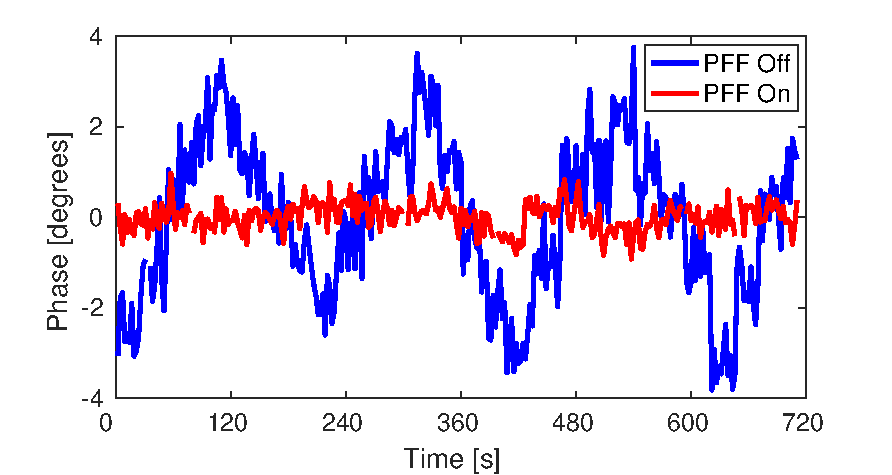
\includegraphics[width=\columnwidth]{figs/wiggle}
	\caption{\label{fig:wiggle}Mean downstream phase with the PFF system off 
		(blue) and on (red) vs. time, with additional phase variations added to 
		the 
		incoming phase.}
\end{figure}

To conclude, CLIC requires a PFF system to reduce the drive beam phase jitter 
by an order of magnitude, from \(2.0^\circ\) to \(0.2^\circ\)~at~12~GHz, or 
better than 50~fs stability. A prototype of the system has been 
in operation at the CLIC test facility CTF3, and corrects the beam phase by 
varying the path length through a chicane using two electromagnetic kickers. 
As well as the kickers, the system uses newly designed phase monitors with 
\(0.12^\circ\) resolution, high bandwidth 20~kW amplifiers and a low latency 
digitiser/feedforward controller. The system latency, including hardware and 
signal transit times, is less than the 380~ns beam time of flight between the 
input phase monitor and the correction chicane. Therefore, the feedforward 
correction can be directly applied to the same bunch initially measured at the 
monitor. New optics for the correction chicane and other beam lines at CTF3 
have been 
developed to yield the desired phase shifting behaviour and ensure high 
correlation between the initial upstream and downstream phase.

The prototype system has demonstrated \(0.20\pm0.01^\circ\) pulse-to-pulse 
phase jitter on a time scale of ten minutes, verifying the feasibility of the 
concept. It has also been shown to be able 
to flatten intra-pulse phase variations up to a frequency of 25~MHz. On longer 
timescales the performance of the system is limited by changes to the incoming 
beam conditions, in particular beam energy, which would be better controlled in 
any future application at CLIC.

\begin{acknowledgments}
	We wish to acknowledge Alessandro Zolla and Giancarlo Sensolini (INFN 
	Frascati) for their work on the mechanical design of the phase monitors and 
	kickers, 
	Alexandra Andersson, Luca Timeo and Stephane Rey (CERN) for their work on 
	the phase monitor electronics, and everyone involved in the operation of 
	CTF3 for their help and support in realising the PFF system.
\end{acknowledgments}

\bibliography{pff_short}

\end{document}
